\documentclass[openany,oneside]{ctexbook}
\usepackage{amsfonts}  %oneside为单面输出

%============================ 引用的宏包 ==================================%

\usepackage{booktabs}  %可以使用命令\specialrule改变表中线的粗细
\usepackage{CJK,CJKnumb}  %调用中日韩字库包
\usepackage{graphicx}  %插入图需要
\usepackage{bm}         % 处理数学公式中的黑斜体的宏包
\usepackage{amsmath}    % AMSLaTeX宏包 用来排出更加漂亮的公式
\usepackage{amssymb}    % AMSLaTeX宏包 用来排出更加漂亮的公式
\usepackage{color}   %控制颜色的
\usepackage{a0size}     %自由定义字号,在后面“字号设置”中可设置到107pt 为止的大字体
\usepackage{titletoc}  %设计目录的格式
\usepackage{titlesec}  %设计标题的格式
\usepackage{cases}  %这个包有时会起副作用, 尽量避免使用
\usepackage{fancyhdr}  %可用来灵活设置页眉和页脚
\pagestyle{fancy}
\fancyhf{}
\fancyhead[C]{\thepage}
\usepackage{enumerate} %清单明细专用
\usepackage{appendix}  %附录专用
\usepackage{cite}%产生如(文[2,4-8])的效果
\usepackage{multirow}
%\usepackage{amsthm}
\usepackage{CJK}
\usepackage{epstopdf}
\usepackage{listings} %新加入的宏包,用于附录插入代码
\usepackage{graphicx}
\usepackage{subfigure}
\usepackage{float}
\lstset{
    basicstyle=\small,
    numbers=left,
    numberstyle=\tiny,
    stepnumber=1,
    numbersep=5pt,
    language=Python,
    escapeinside=``,
    extendedchars=false,
    showspaces=false
}
\usepackage{float,graphicx}
\usepackage[font=normalsize,labelfont=bf,textfont=bf]{caption}  %图标的标题字体和自号
%\usepackage[font=normalsize,labelfont=normalsize,textfont=normalsize]{caption}  % 图标的标题字体和自号
\DeclareCaptionLabelSeparator{twospace}{\ ~}  %将图表标题中的冒号改成空格
\captionsetup{labelsep=twospace}


\textwidth 159mm %设置版面宽度
\textheight 225mm %设置版面高度
\topmargin -5mm %设置页面顶端空白的高度
\oddsidemargin 5mm %设置奇数页的边距
\evensidemargin 5mm  %设置偶数页的边距, 单面时不起作用
\renewcommand\baselinestretch{1.5} %将文本的行间距设为基础行间距的1.5 倍
\renewcommand\arraystretch{1} %将数组中的行间距设为基础行间距的2 倍
\newcommand{\upcite}[1]{\textsuperscript{\textsuperscript{\cite{#1}}}}
  % 将引用的参考文献标号显示为上标
\setlength{\parskip}{3pt plus1pt minus1pt}  % 段落之间的竖直距离



\begin{document}
  
%===================== 重定义字体、字号命令 =============================%
% 注意win2000,没有 simsun, 最好到网上找一个. 一些字体是office2000 带的
\newcommand{\song}{\CJKfamily{song}}    % 宋体   (Windows自带simsun.ttf)
\newcommand{\fs}{\CJKfamily{fs}}        % 仿宋体 (Windows自带simfs.ttf)
\newcommand{\kai}{\CJKfamily{kai}}      % 楷体   (Windows自带simkai.ttf)
\newcommand{\hei}{\CJKfamily{hei}}      % 黑体   (Windows自带simhei.ttf)
\newcommand{\li}{\CJKfamily{li}}        % 隶书   (Windows自带simli.ttf)
\newcommand{\you}{\CJKfamily{you}}      % 幼圆   (Windows自带simyou.ttf)
\newcommand{\chuhao}{\fontsize{42pt}{\baselineskip}\selectfont}     % 字号设置
\newcommand{\xiaochuhao}{\fontsize{36pt}{\baselineskip}\selectfont} % 字号设置
\newcommand{\yihao}{\fontsize{28pt}{\baselineskip}\selectfont}      % 字号设置
\newcommand{\erhao}{\fontsize{21pt}{\baselineskip}\selectfont}      % 字号设置
\newcommand{\xiaoerhao}{\fontsize{18pt}{\baselineskip}\selectfont}  % 字号设置
\newcommand{\sanhao}{\fontsize{15.75pt}{\baselineskip}\selectfont}  % 字号设置
\newcommand{\xiaosanhao}{\fontsize{14.75pt}{\baselineskip}\selectfont}  % 字号设置
\newcommand{\sihao}{\fontsize{14pt}{\baselineskip}\selectfont}      % 字号设置
%\newcommand{\xiaosihao}{\fontsize{12pt}{20pt}\selectfont}  % 字号设置
\newcommand{\xiaosihao}{\fontsize{12pt}{14pt}\selectfont}  % 字号设置
\newcommand{\wuhao}{\fontsize{10.5pt}{12.6pt}\selectfont}    % 字号设置
\newcommand{\xiaowuhao}{\fontsize{9pt}{11pt}{\baselineskip}\selectfont}   % 字号设置
\newcommand{\liuhao}{\fontsize{7.875pt}{\baselineskip}\selectfont}  % 字号设置
\newcommand{\qihao}{\fontsize{5.25pt}{\baselineskip}\selectfont}    % 字号设置

%\theoremstyle{plain}
%\newtheorem{theorem}{定理}[section]  %显示定理2.4.1  (2.4节的第1个定理)
\newtheorem{theorem}{定理}[chapter]  %显示定理2.1.  (第2章的第1个定理)
\newtheorem{definition}{定义}[chapter]
\newtheorem{remark}{注}[chapter]
\newtheorem{example}{例}[chapter]
\newtheorem{corollary}{推论}[chapter]
\newtheorem{proposition}{命题}[chapter]
\newtheorem{lemma}{引理}[chapter]
\newtheorem{assumption}{假设}[chapter]

\def\proof{\indent{\hei 证明\ \ } \ignorespaces}
\def\endproof{\vbox{\hrule height0.6pt\hbox{\vrule height1.3ex width0.6pt\hskip0.8ex\vrule width0.6pt}
               \hrule height0.6pt}\vskip 3mm}

\catcode`@=11

% Change definition of \thebibliography environment to use smaller font.
\renewenvironment{thebibliography}[1]
     {\def\chaptername{}\chapter{\bibname}
     %\thispagestyle{headings}  %使参考文献列表的起始页显示页眉                            !!!
      \list{\@biblabel{\@arabic\c@enumiv}}%
           {\settowidth\labelwidth{\@biblabel{#1}}%
            \leftmargin\labelwidth
            \advance\leftmargin\labelsep
            \@openbib@code
            \usecounter{enumiv}%
            \let\p@enumiv\@empty
            \renewcommand\theenumiv{\@arabic\c@enumiv}}%
      \small%                                               !!!
      \sloppy
      \clubpenalty4000
      \@clubpenalty \clubpenalty
      \widowpenalty4000%
      \sfcode`\.\@m}
     {\def\@noitemerr
       {\@latex@warning{Empty `thebibliography' environment}}%
      \endlist}

%%%%%%%%%%%%%%%%%%%%%%%%%%%开始章的定义%%%%%%%%%%%%%%%%%%%%%%%%%%%%%%

% Define chapter
\renewcommand\chaptername{第\thechapter章}
\def\@chapter[#1]#2{\ifnum \c@secnumdepth >\m@ne
                           %\pagestyle{empty}%                       !!!
                       \if@mainmatter
                           \pagestyle{headings}%                       !!!
                           \refstepcounter{chapter}%
                          \protected@xdef\@currentlabel{\chaptername}%  !!!
                          \typeout{\hei\erhao \@chapapp \space \thechapter.}%
                          \addcontentsline{toc}{chapter}{\protect\numberline
                          {\hei\xiaosihao\chaptername} {\hei\xiaosihao #1}}%  !!!
                       \else
                          \addcontentsline{toc}{chapter}{\hei\xiaosihao #1}%
                       \fi
                    \else
                       \addcontentsline{toc}{chapter}{\xiaosihao #1}%
                    \fi
                    \chaptermark{#1}%
                    \addtocontents{lof}{\protect\addvspace{10\p@}}%
                    \addtocontents{lot}{\protect\addvspace{10\p@}}%
                    \if@twocolumn
                       \@topnewpage[\@makechapterhead{#2}]%
                    \else
                       \@makechapterhead{#2}%
                       \@afterheading
                    \fi
                    }
\def\@chapapp{Chapter}%                   !!!
\def\chapterformat{\xiaoerhao\bfseries\centering}%      |||
\def\@makechapterhead#1{%
                \if@mainmatter
                          \renewcommand\leftmark{\wuhao \chaptername\ \ \ #1}
                       \else
                          \renewcommand\leftmark{\wuhao #1}%
                       \fi
                         \vspace*{-\headsep}\vspace*{-\headheight}\vspace*{15\p@}%      !!!
                         {\chapterformat%                       !!!
                         \ifnum \c@secnumdepth >\m@ne%                                !!!
                             \if@mainmatter%                                            !!!
                                \chaptername \quad #1 \par\nobreak%      !!!
                             \else%                                                     !!!
                                #1 \par\nobreak%                         !!!
                             \fi%                                                       !!!
                         \fi%                                                         !!!
                         \vskip 15\p@%                                                !!!
                         }
                        }
\def\@makeschapterhead#1{%
                            \vspace*{-\headsep}\vspace*{-\headheight}\vspace*{15\p@}%   !!!
                            {\chapterformat%                        !!!
                             \interlinepenalty\@M%                                     !!!
                             #1\par\nobreak%                                           !!!
                             \vskip 15\p@%                                             !!!
                            }
                         }
%%%%%%%%%%%%%%%%%%%%%%%%%%%结束章的定义%%%%%%%%%%%%%%%%%%%%%%%%%%%%%%

\renewcommand \thetable
     {\ifnum \c@chapter>\z@ \thechapter -\fi \@arabic\c@table}  %定义表的编号形式

\renewcommand \thefigure
     {\ifnum \c@chapter>\z@ \thechapter -\fi \@arabic\c@figure}  % 定义图的编号形式


\catcode`@=12


% \titleformat{\chapter}{\sffamily\centering\hei\sihao }{\chaptername}{.8em}{}
% \titlespacing{\chapter}{0pt}{*1}{*1}  %定义一级标题的格式
%   \titleformat{\section}{\sffamily\CJKfamily{hei}\xiaosihao }{\hspace*{0.8cm}\thesection }{.8em}{} %定义二级标题的格式
% \titleformat{\subsection}{ \sffamily\CJKfamily{hei}\xiaosihao }{ \hspace*{0.8cm}\thesubsection }{.8em}{} %定义三级标题的格式
% \titleformat{\subsubsection}{ \sffamily\CJKfamily{hei}\large }{ \hspace*{0.8cm}\thesubsubsection }{.8em}{}  %定义四级标题的格式

\makeatletter
\newcommand\Csub{\@startsection{subsection}{2}%
 {0pt}{-\baselineskip}{.2\baselineskip}%
 {\centering\itshape}}
\newcommand\Lsub{\@startsection{subsection}{2}%
 {0pt}{-\baselineskip}{.2\baselineskip}%
 {\raggedright\sffamily}}
\newcommand\Rsub{\@startsection{subsection}{2}%
 {0pt}{-\baselineskip}{.2\baselineskip}%
 {\raggedleft\MakeUppercase}}
\newcommand\Hsub{\@startsection{subsection}{2}%
 {0pt}{-\baselineskip}{.2\baselineskip}%
 {\hrule\medskip\itshape}}
\makeatother

\pagestyle{empty} %从现在开始页眉为空

\mainmatter
\frontmatter
\renewcommand{\thepage}{\arabic{page}} %从正文开始页号显示为阿拉伯数字



\setcounter{page}{1}


\chapter{\sihao\hei \quad 建模国家中心城市格局}
\begin{center}
   
      {\textbf{\sihao\hei \quad 一\quad 摘要}}
\end{center}
本文主要分析了我国中心城市的评选
指标,研究了具体应该设立多少个中心城市
以及设立哪些城市为中心城市最有利于
国家发展,并且预测了在2035年我国中
心城市的格局。建立了层次分析模型、层
次聚类模型以及回归模型。

问题一,对于中心城市的评选标准的评价指标本文主要考虑了包括地区生产总值、地方财政收入、人口总数等五个指标。
建立层次分析模型,通过一致性检验后得出
各个评价指标的相应权重以及目前各个城市在这五个指标上的加权得分值。

问题二,中心城市设立过多或者过少均不利于国家发展,考虑到中心城市的在经济、人口、就业等方面的相似程度,建立层次聚类模型将
所有城市分成两类即中心城市与非中心城市,在中心城市这一类中城市的数量取为当前我国最适合设立中心城市的个数。
根据聚类图的结果得出我国目前应该设立11个中心城市最有利于国家发展。这十一个城市分别是南京、成都、天津、
广州、上海、北京、西安、重庆、武汉、沈阳、郑州,排名不分先后。




问题三,中心城市必然会随着经济等形势的变化而变化,对于问题三建立回归模型预测各个城市在2035年的评价指标值,
问题一中已经利用层次分析法给出这些指标的相应权重值,在假设2035年这些指标权重值仍然不变的情况下通过加权求出分数值便
可以判断出在2035年我国中心城市的格局。
根据本文预测的结果,南京、沈阳、厦门三个城市按照本文预测的结果可以在2035年跻身在国家中心城市之内,而
郑州在2035年可能在这五个准则标准中达不到中心城市的水准。

问题四,我们认为应该着重发展南京、沈阳、厦门这三个城市。因为无论是根据
聚类的结果还是预测的结果,这三个城市在这五个准则指标下均可以达到国家中心的水准。

{\bfseries 关键词}:中心城市; 层次分析模型; 聚类; 回归分析;

\chapter{\sihao\hei 二\quad 问题分析}
{\bfseries 问题背景}:

国家发展改革委在2016年《关于支持武汉建设国家中心城市的指导意见》中明确指出,
国家中心城市是指居于国家战略要津、肩负国家使命、
引领区域发展、参与国际竞争、代表国家形象的现代化大都市。在资
源环境承载条件和经济发展基础较好的地区规划建设国家中心城市,
既是引领全国新型城镇化建设的重要抓手
,也是完善对外开放区域布局的重要举措。
2010年,住建部发布的《全国城镇体系规划(2010-2020年)》中首次提出建设北
京、天津、上海、广州、重庆五大国家中心城市。2016年5月发
布的《成渝城市群发展规划》,明确成都要“以建设国家中心城市为目标”。2016
年12月份,国家发改委发布《促进中部地区崛起“十三五”规划》,明确支持武
汉、郑州建设国家中心城市。2018年2月份发布的《关中平原城市
群发展规划》明确提出“建设西安国家中心城市”。至此,我国已有9
座城市进入国家中心城市建设之列。
作为我国城镇体系层级的“塔尖”,目前
我国已有北京、天津、
上海、广州、重庆、成都、武汉、郑州、西安9座城市被
明确定位为国家中心城市。



{\bfseries 问题一分析}:

针对问题一,可以考虑地区生产总值、人口总数、财政收入等几个常用评价
指标建立层次分析模型,因为它特别适用于那些难于完全定量分析的问题。设定好评价准则以及判别矩阵,如果通过一致性检验便
可以得到各个评选标准对应的权重。

{\bfseries 问题二分析}:
针对问题二,由于评定中心城市是由相同的指标因素来评定的,所以在这几个指标上中心城市会比非中心城市相似度更大,鉴于这一点
可以建立层次聚类模型将中心城市聚为一类以此分析哪些城市应该算是中心城市。


{\bfseries 问题三分析}:

根据上述查阅的数据,将时间作为自变量,也成为回归变量,五个评价准则分别作
为因变量建立多个回归模型分别预测出在2035年各个城市的这五个评价准则的预测值然后代入上述建立的层次
分析模型,假设在每一个准则所对应的权值仍然不变,那么便可以计算出在2035年哪些城市符合国家中心城市的评选标准。

\chapter{\sihao\hei 三\quad 模型假设与符号说明}

\begin{center}
  \bf{模型假设}
\end{center}

\begin{enumerate}
  \item 假设在2035年各个城市内国家重点高校数量不变
  \item 假设在2035年各个准则指标权值不变
\end{enumerate}

\begin{center}
  \bf{符号说明}
\end{center}

\begin{table}[!htp]
  \centering
  \begin{tabular}{|l|c|}
    \hline
    $X_1$&人口总数 \\ \hline
    $X_2$&地区生产总值 \\ \hline
    $X_3$&国家重点高校数量 \\ \hline
    $X_4$&地方财政收入 \\ \hline
    $X_5$&人均可支配收入 \\ \hline
    $\hat{{\sigma}^*}^2$&$\displaystyle\frac{1}{n-2}\displaystyle\sum_{i=1}^{n}{(y_i-\hat{y_i})}^2$\\ \hline
    
    $D_{ij}$&$\min\{d_{ij}|x_{i} \in G_p,x_j \in G_q\}$类间最短距离 \\ \hline
  
  
  
   \end{tabular}
\end{table}


\chapter{\sihao\hei 四\quad 模型的建立与求解}

{\bfseries 问题一的求解}:

针对问题一,本文考虑的评价指标包括地区生产总值、地方财政收入、人口总数等五个指标,
建立层次分析模型。层次分析法是一种定性和定量相结合的、系统的、层次化的分析方法。建模步骤如下:



{\bfseries 1. 将因素分层}

\begin{enumerate}
   \item 目标层:中心城市的评选标准
   \item 准则层:上述所提到的地区生产总值、人口总数等五个评价因素
   \item 方案层:备选中心城市
\end{enumerate}

{\bfseries 2. 构造判别矩阵}

层次结构反映了因素之间的关系,但准则层中的各准则在目标衡
量中所占的比重
并不一定相同,在决策者的心目中,它们各占有一定的比例。构造判别矩阵的方法为:反复咨询专家然后根据各个
准则因素,对元素两两比较哪个重要,重要多少,对重要程度按$1-9$赋值如下表:

\begin{center}
   \textbf{重要性标度含义表}
\end{center}

\begin{table}[!htp]
   \centering
   \begin{tabular}{l|c}
      \hline
      重要性标度&含义 \\ \hline
      1&表示两个元素相比较,具有同等重要性 \\ \hline
      3&表示两个元素相比较,前者比后者稍重要 \\ \hline
      5&表示两个元素相比较,前者比后者明显重要 \\\hline
      7&表示两个元素相比较,前者比后者强烈重要 \\\hline
      9&表示两个元素相比较,前者比后者极端重要 \\\hline
      2,4,6,8&表示上述判断的中间值 \\\hline
      
   \end{tabular}
\end{table}


显然判别矩阵具有反对称性。在使用判断矩阵求权重之前,必须对其进行一致性检验。
%9个这样的矩阵才行

{\bfseries 3. 计算权向量与判别矩阵的一致性检验}


本文计算权向量采用和法,具体步骤如下:
\begin{enumerate}
   \item 将判别矩阵按列归一化:$b_{ij}=\displaystyle\frac{a_{ij}}{\displaystyle\sum_{i=1}^{n}a_{ij}}$
   \item 按行求和:$v_i=\displaystyle\sum_{j=1}^{n}b_{ij}$
   \item 归一化:$w_i=\displaystyle\frac{v_i}{\displaystyle\sum_{i=1}^{n}v_i}$,即为近似权向量
   \item 为了进行一致性检验,求最大化特征根 $\lambda_{max}=\displaystyle\frac{1}{n}\displaystyle\sum_{i=1}^{n}\displaystyle\frac{(Aw)_{i}}{w_i}$
\end{enumerate}

{\bfseries 一致性检验}:
\begin{enumerate}
   \item 计算一致性指标$CI(consistency index)$,$CI=\displaystyle\frac{\lambda_{max}-n}{n-1}$
   \item 查表确定相应的平均随机一致性指标$RI(random index)$
   \item 计算一致性比例$CR(consistency ratio)$,$CR=\displaystyle\frac{CI}{RI}$
\end{enumerate}

\pagestyle{plain}



当$CR=0$时,认为判别矩阵具有完全一致性,当$CR<0.1$时,认为判别矩阵的一致性可以接受,
当$CR>0.1$时,认为判别矩阵不符合一致性要求需要对判别矩阵重新构造,加以修正。

\begin{table}[!htp]
   \centering
   \begin{tabular}{|l|c|c|c|c|c|}
      \hline
      &$X_1$&$X_2$&$X_3$&$X_4$&$X_5$\\ \hline
      $X_1$&1&$\displaystyle\frac{1}{6}$&3&2&4 \\ \hline
      $X_2$&6&1&9&9&9 \\ \hline
      $X_3$&$\displaystyle\frac{1}{3}$&$\displaystyle\frac{1}{9}$&1&$\displaystyle\frac{2}{3}$&$\displaystyle\frac{4}{3}$ \\ \hline
      $X_4$&$\displaystyle\frac{1}{2}$&$\displaystyle\frac{1}{9}$&$\displaystyle\frac{3}{2}$&1&2 \\ \hline
      $X_5$&$\displaystyle\frac{1}{4}$&$\displaystyle\frac{1}{9}$&$\displaystyle\frac{3}{4}$&$\displaystyle\frac{1}{2}$&1 \\ \hline
   \end{tabular}
   \caption{目标层到准则层的判别矩阵}
\end{table}

上表就是目标层到准则层的判别矩阵,利用上述所讲的模型计算步骤,利用Python编程得到结果
\[
   CR=0.0265,\qquad w=[0.184\quad 0.614\quad 0.062\quad  0.092\quad 0.047]
\]
$CR=0.0265<0.1$,模型通过一致性检验且由计算得到的特征向量可见各个准则因素所占权重的比例由大到小依次为$X_2,X_1,X_4,X_3,X_5$。

进一步,通过查阅资料得到近几年来各个备选中心城市的以上五个评价准则因素的数据
,为了计算简便起见,本文将这几年的数据取平均值然后构造
了准则层到决策层的一共5个$9\times 9$的判别矩阵。利用上述模型分别对这5个判别
矩阵进行层次分析,
最终得到每一个备选中心城市对应的权重以及相应的得分见下表2。

\begin{table}[!htp]
   \centering
   \begin{tabular}{|l|c|c|c|c|c|c|c|c|c|c|}
      \hline
      &指标权重&北京&天津&上海&广州&重庆&成都&武汉&郑州&西安 \\ \hline
      $X_1$&0.18379&0.14181&0.1027&0.15958&0.09545&0.20422&0.09717&0.07169&0.06669&0.0607 \\ \hline
      $X_2$&0.61445&0.17374&0.1078&0.1875&0.13131&0.11697&0.08773&0.08486&0.0625&0.04759 \\ \hline
      $X_3$&0.06225&0.35789&0.05263&0.13684&0.16842&0.02105&0.07368&0.09474&0.01053&0.08421 \\ \hline
      $X_4$&0.09237&0.20994&0.07244&0.25792&0.09854&0.08222&0.05168&0.10523&0.06905&0.05299 \\ \hline
      $X_5$&0.04718&0.15979&0.10123&0.16446&0.14118&0.06761&0.09261&0.10796&0.08469&0.08048 \\ \hline
   \end{tabular}
   \caption{目前九个中心城市在这五个评价指标上的权重}
\end{table}

最终得到每一个城市在这五个指标权重上的得分如表3
\begin{table}[!htp]
   \centering
   \begin{tabular}{|l|c|}
      \hline
      &加权得分值 \\ \hline
      北京&0.182 \\ \hline
      上海&0.184 \\ \hline
      天津&0.099 \\ \hline
      广州&0.124 \\ \hline
      重庆&0.122 \\ \hline
      成都&0.085 \\ \hline
      武汉&0.086 \\ \hline
      郑州&0.062 \\ \hline
      西安&0.054 \\ \hline
      
   \end{tabular}
   \caption{九个中心城市在这五个评价指标下的综合加权得分}
\end{table}

{\bfseries 问题二的求解}:

考虑到各个中心城市在各个评选指标上的相似程度,建立层次聚类模型。
聚类的迭代过程可以总结如下:
\begin{enumerate}
   \item 计算$n$个样本两两之间的欧氏距离,记作距离矩阵$D=[d_{ij}]$
   \item 构造$n$个类,每一类仅仅包含一个样本
   \item 合并类间距离最小的两个类,其中最短距离为类间距离,构造一个新类
   \item 计算新类与当前各个类之间的距离,若类的个数为1则终止计算,否则回到步骤3
   
\end{enumerate}

为了简便,本文共考虑了15个城市,分别是北京、
上海、
重庆、
天津、
广州、
成都、
武汉、
郑州、
西安、
南京、
厦门、青岛、哈尔滨、合肥、沈阳。可以看作15个样本,以人口总数、地区生产总值等上述五个评价指标作为这些样本的特征。
具体数值详见附录。通过这些数据得到样本与样本之间的距离矩阵如下:

利用Python编程并且画出聚类图如图所示

\begin{figure}[htp]
   \centering
   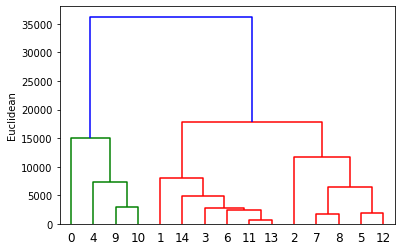
\includegraphics[scale=0.8]{cluster.png}
   \caption{聚类图}
\end{figure}

其中看出数据被大致分成了两类,
其中红色线所代表的类别为中心城市类别,
下方横坐标数字分别对应南京、成都、天津、
广州、上海、北京、西安、重庆、武汉、沈阳、郑州。
绿色线所代表的类别为非中心城市类别包括青岛、合肥、哈尔滨、厦门。
因此根据聚类图可以看出目前国内的城市在这五个指标上可以达到近似的一共有十一个城市。




{\bfseries 问题三的求解}:

以时间作为自变量,也称为回归变量,四个评价准则分别作
为因变量建立多个回归模型分别预测出在2035年各个城市的这
四个评价准则的预测值。其中重点高校数量与时间变量没有线性相关性,本文假设在2035年各个城市的重点高校数量不变。


一般的称下式所确定的模型为一元线性回归模型
\[
   \left\{\begin{matrix}
      y=\beta_0+\beta_1 x+\epsilon\\ 
      E\epsilon=0,D\epsilon={\sigma}^2
      \end{matrix}\right.
\]

由上式对$y=\beta_0+\beta_1 x+\epsilon$取期望即得到$Y=\beta_0+\beta_1 x$,称为$y$对$x$的回归方程。$\beta_0$和$\beta_1$是回归系数。
常用最小二乘估计来估计回归系数。即对于$\beta_0,\beta_1$有:
\[
   \hat{\beta_0}=\overline{y}-\hat{\beta_1}\overline{x},\quad \hat{\beta_1}=\displaystyle\frac{\displaystyle\sum_{i=1}^{n}(x_{i}-\overline{x})(y_{i}-\overline{y})}{\displaystyle\sum_{i=1}^{n}{(x_i-\overline{x})}^2}
\]
当求出回归方程后需要对回归系数做显著性检验。
\[
   H_0:\hat{\beta_1}=0,\quad H_1: \hat{\beta_1}\neq 0
\]
构造统计量
\[
   T=\displaystyle\frac{\hat{\beta_1}}{\hat{{}\sigma}^*}\sqrt{\displaystyle\sum_{i=1}^{n}{(x_i-\overline{x})}^2}
\]
且$T \sim t(n-2)$。本文预测15个城市的未来的评价指标因此$n=15$。
对于给定显著性水平$\alpha$,查找分位数$t_{\alpha/2}(n-2)$。本文取$\alpha=0.5$,因此即查找$t_{0.025}(13)=2.1604$
在给定的一组回归值代入统计量中若$|t|\geqslant 2.1604$则拒绝$H_0$,否则接受$H_0$。
预测的结果见表4。根据所预测的数值与问题一中已经求解的指标的权值对应相乘得到结果如表5。

\begin{table}[!htp]
   \centering
   \begin{tabular}{|l|c|c|c|c|c|}
      \hline
      &$X_1$(万人)&$X_2$(万亿元)&$X_3$(个)&$X_4$(亿元)&$X_5$(元)\\ \hline
      北京&3224.423&5.339&34&11872.339&108815.781 \\ \hline
      天津&2280.827&3.76&5&3599.236&71202.029 \\ \hline
      成都&1525.19&2.361&7&2497.887&74478.789 \\ \hline
      重庆&2957.995&3.678&2&4880.363&51967.955 \\ \hline
      西安&917.135&1.111&8&2568.756&55064.852 \\ \hline
      沈阳&928.997&1.23&3&1339.304&80367.683 \\ \hline
      郑州&1881.6&1.775&1&3536.461&55040.712 \\ \hline
      武汉&1141.491&1.823&9&3061.692&79424.396 \\ \hline
      南京&1075.479&2.435&10&2289.361&70157.386 \\ \hline
      厦门&611.506&1.148&1&2372.302&83356.544 \\ \hline
      上海&3549.8&5.657&13&14654.057&60844.882 \\ \hline
      合肥&598.547&1.025&1&1247.245&63214.547 \\ \hline
      广州&3124.887&4.258&6&10245.52&72548.667 \\ \hline
      青岛&658.546&0.878&2&1178.658&59877.634 \\ \hline
      哈尔滨&879.258&0.997&5&1254.984&72546.335 \\ \hline

      
   \end{tabular}
   \caption{2035年部分城市的中心城市评价指标预测}

\end{table}


\begin{table}[!htp]
   \centering
   \begin{tabular}{|l|c|}
      \hline

      北京&6828.590 \\ \hline
      上海&4113.587 \\ \hline
      重庆&4026.840 \\ \hline
      天津&3448.681 \\ \hline
      广州&4004.976 \\ \hline
      成都&4087.141 \\ \hline
      武汉&3270.455 \\ \hline
      郑州&3241.5265 \\ \hline
      西安&3721.27 \\ \hline
      南京&4065.047 \\ \hline
      厦门&3880.95 \\ \hline
      青岛&3208.369 \\ \hline
      哈尔滨&3246.537 \\ \hline
      合肥&3055.597 \\ \hline
      沈阳&3901.181 \\ \hline
   \end{tabular}
   \caption{2035年15个城市在指标权重不变的情况下所得的分值}
   
\end{table}
按照分值由高到低的顺序为北京、上海、重庆、南京、成都、广州、
沈阳、厦门、西安、天津、武汉、郑州、哈尔滨、青岛、合肥。
由此,如果仍以11个中心城市为标准的话,那么前十一个城市分别是北京、上海、重庆、南京、成都、广州、
沈阳、厦门、西安、天津、武汉。

可以看出南京、沈阳、厦门三个城市按照本文预测的结果可以在2035年跻身在国家中心城市之内,而
郑州在2035年可能在这五个准则标准中达不到中心城市的水准。


{\bfseries 问题四的求解}:

近年来把“万亿元GDP”作为衡量国家中心城市主要标准的说
法在社会上广为流传,不仅直接影响到个别入选城
市的发展思路和规划编制,也在一些有竞争力的大
城市之间掀起了新一轮的“GDP”竞赛。但这个流行说法,在住房
城乡建设部和国家发展改革委两方面均找不到任何依据。受其影响,一些大城
市把心思和精力主要用于提升自身的首位度上,背弃了中心城市
加强了对周边中小城市的截留、虹吸和压制。应尽快明确国家中心城市的核心
职能,承担国家战略使命和战略意图,促进国家中心城市的健康培育和成长。
因此本文考虑了五个评选准则因素并且进行加权求和得出最后的分值,
我们认为应该着重发展南京、沈阳、厦门这三个城市。因为无论是根据
聚类的结果还是预测的结果,这三个城市在这五个准则指标下均可以达到国家中心的水准。






\begin{thebibliography}{99}

   \bibitem{k0}
   \newblock 中国统计年鉴2018.
   \newblock  http://www.stats.gov.cn/tjsj/ndsj/2018/indexch.htm.
   
   
   \bibitem{k3}
   司守奎,孙兆亮.
   \newblock 数学建模算法与应用.
   \newblock 国防工业出版社.
   \newblock 2015(4): 150-156.
   
   \bibitem{k4}
   塞巴斯蒂安·拉施卡(Sebastian Raschka).
   \newblock Python机器学习.
   \newblock 机器工业出版社.
   \newblock 2017(3): 56-65.
   
   
   
   
   
   
   
   \end{thebibliography}


\chapter{附录}\label{note}

\begin{appendix}
   \subsubsection{判别矩阵的的权值计算以及一致性检验}
   \begin{lstlisting}[firstnumber=1]
      import numpy as np
      A=np.array([[1,1/6,3,2,4],[6,1,9,9,9],[1/3,1/9,1,2/3,4/3],[1/2,1/9,3/2,1,2],[1/4,1/9,3/4,1/2,1]])
      B=A/np.sum([np.transpose(A)[i] for i in range(5)])#因为是对列归一化,所以取先取转置
      v=np.zeros(5)
      for i in range(5):
         v[i]=np.sum([B[i][j] for j in range(5)])
      w=v/np.sum(v)
      lambda_max=np.sum(A.dot(w)/w)/5
      print(lambda_max)#5.11836095 这就是最大特征根
      print(w)#[0.18373494 0.61445783 0.062249   0.09236948 0.04718876] 特征向量
      CI=(lambda_max-5)/(5-1)
      RI=1.12#查表得到的,如果n==9 则RI=1.46
      CR=CI/RI
      if CR<0.1:
         print("通过一致性检验")
      else:
         print("未通过一致性检验,需要重新修改判别矩阵")
      
   \end{lstlisting}

   \subsubsection{准则层到目标层的权值向量的计算}
   \begin{lstlisting}[firstnumber=1]
      human_amount=[2154,1560,2424,1449.84,3102,1476,1089,1013,922]#九个中心城市的人口总数
      gdp=[3.03,1.88,3.27,2.29,2.04,1.53,1.48,1.09,0.83]#九个中心城市的GDP
      university=[34,5,13,16,2,7,9,1,8]#九个中心城市的重点高校数量
      finance_revenue=[5785.9,1996.3,7108.1,2715.6,2266,1424.2,2900,1903,1460.39]#九个中心城市的财政收入
      per_personl=[62361,39506,64183,55099,26386,36142,42133,33051,31407]#九个中心城市的人均可支配收入
      import numpy as np
      def get_judge_matrix(judge_baseline):
         length=len(judge_baseline)
         judge_matrix=np.identity(length)
         for i in range(length):
            value=judge_baseline[i]
            for j in range(length):
                  judge_matrix[i][j]=value/judge_baseline[j]
                  judge_matrix[j][i]=judge_baseline[j]/value
         return judge_matrix#返回判别矩阵
      human_amount_matrix=get_judge_matrix(human_amount)
      gdp_matrix=get_judge_matrix(gdp)
      university_matrix=get_judge_matrix(university)
      finance_revenue_matrix=get_judge_matrix(finance_revenue)
      per_personl_matrix=get_judge_matrix(per_personl)
      #现在已经得到了各个评价准则指标的判别矩阵,下面计算权值向量,
      def get_weights_vector(judge_matrix):
         length=judge_matrix.shape[0]
         B=judge_matrix/np.sum([np.transpose(judge_matrix)[i] for i in range(length)])
         V=np.sum([judge_matrix[i] for i in range(length)],axis=1)#按行求和
         W=V/np.sum(V)#归一化
         lambda_max=np.sum(judge_matrix.dot(W)/W)/5
         return W
      

   \end{lstlisting}

   \subsubsection{利用层次聚类分析中心城市的个数}
   \begin{lstlisting}[firstnumber=1]
      import numpy as np
      import pandas as pd
      from scipy.cluster.hierarchy import dendrogram,linkage
      form scipy.spatial.distance import pdist
      indexs=[str(i) for i in np.arange(len(15))]
      columns=['X_1','X_2','X_3','X_4','X_5']
      X=np.ndarray((20,5))
      df=pd.DataFrame(X,columns=columns,index=indexs)
      clusters=linkage(df.values,method='complete',metric='euclidean')
      #print(pd.DataFrame(clusters,columns=['city_','']))
      dend_gram=dendrogram(clusters,labels=indexs)
      import matplotlib.pyplot as plt
      plt.tight_layout()
      plt.show()


   \end{lstlisting}

\end{appendix}
\subsubsection{回归分析预测2035年各个城市的评价指标值}
\begin{lstlisting}[firstnumber=1]
   import pandas as pd
   from sklearn.linear_model import LinearRegression
   slr=LinearRegression()
   def predict_(criterion_data,slr):
    year_list_=np.reshape(criterion_data[0],(-1,1))
    predict_result=[]
    for data in criterion_data[1:]:
        slr.fit(year_list_,data)
        predict_result.append(slr.coef_[0]*2035+slr.intercept_)
    return predict_result
   predict_result=predict_(criterion_data,slr)
   data=pd.read_excel("./model_data/data.xlsx")#将要读取的数据写成data.xlsx放到data文件夹下

   
\end{lstlisting}





\end{document}


